\documentclass[a4paper,12 pt]{article}
\usepackage{geometry}
\geometry{letterpaper, margin=0.8in}
\usepackage[english]{babel}
\usepackage[utf8]{inputenc}
\usepackage{enumitem}
\setlist{  
  listparindent=\parindent,
  parsep=0pt,
}
\usepackage{amsmath}
\usepackage{graphicx}
\usepackage[colorinlistoftodos]{todonotes}
\usepackage{float}
\usepackage{amssymb}
\usepackage{bbm}
\usepackage[normalem]{ulem}
\usepackage{natbib}
\usepackage{listings}

\newcommand{\mpi}{\texttt{MPI\_Reduce }}
\newcommand{\pp}{\texttt{MPI\_P2P\_reduce }}

\title{\vspace{-2.0cm}CSCI 6360: Parallel Computing Assignment 3 Report}
\author{Anirban Das (dasa2@rpi.edu) }
\date{March 23, 2018}


\begin{document}
\maketitle

\subsection{Graphs}
Here, we are plotting runtimes of both the \mpi and \pp collective operations as a function of the number of ranks. In both cases we assume the runtime equal to the sum of time required to do the local sum and the collective operations. 
\begin{figure}[H]
	\centering
	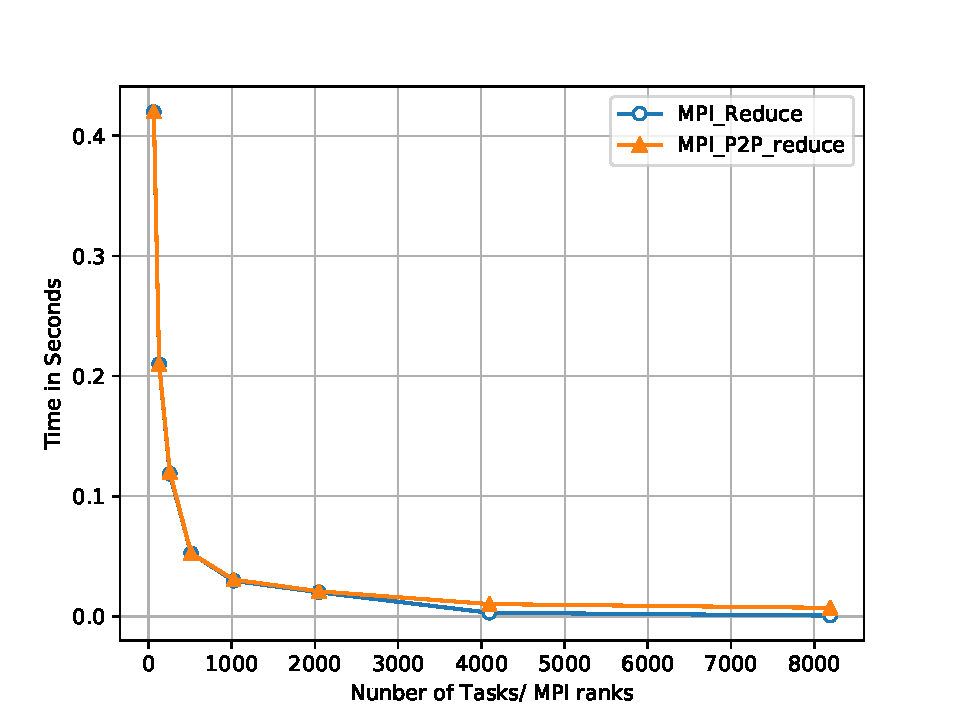
\includegraphics[width=0.8\linewidth]{Graphs/MPI_vs_P2P}
  \caption{Plot the execution time of both reduction approaches as a function of the number of MPI ranks (Y axis in seconds)}
\end{figure}
The following is the same graph, but with a $\pmb{\log_{10}(seconds)}$ Y axis, so that the difference between performance of \mpi and \pp is more prominent:
\begin{figure}[H]
	\centering
	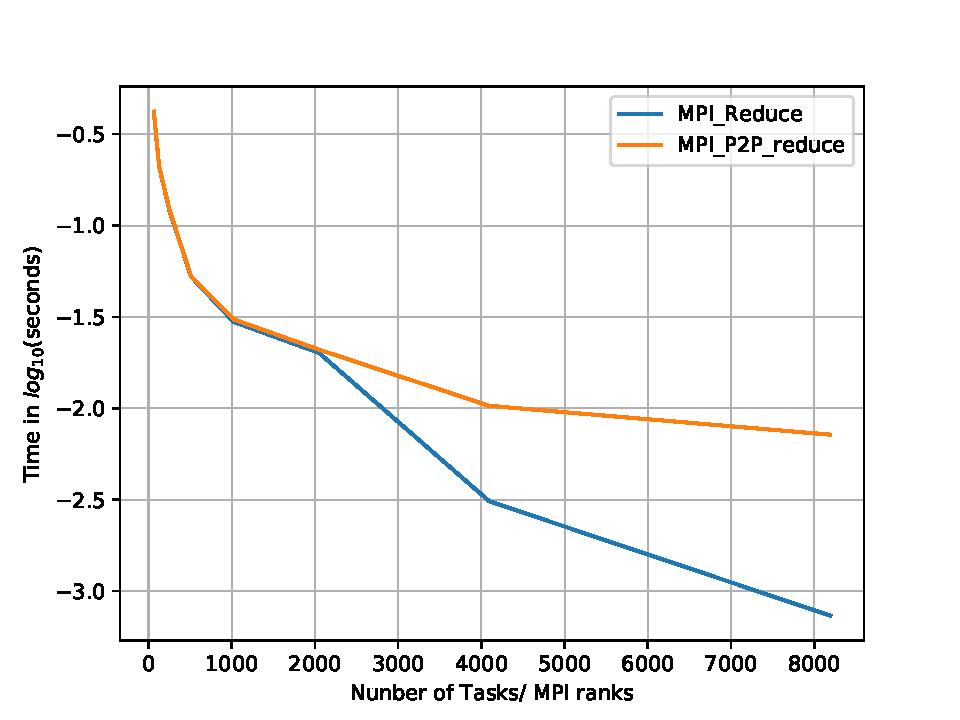
\includegraphics[width=\linewidth]{Graphs/MPI_vs_P2P_log}
  \caption{Plot the execution time of both reduction approaches as a function of the number of MPI ranks (Y axis in log10)}
\end{figure}


\subsection{Observations}
\textbf{First of all, \mpi is always faster than \pp.} This is uniform across all rank runs. 

\begin{enumerate}
\item We observe that with increase in the number of ranks, the runtime goes down for both \mpi and \pp,with the lowest for 8192 MPI ranks. This is partly because of two reasons :
\begin{enumerate}
\item With increase in number of ranks, our 1 billion long array is fragmented up in 8192 small subarrays in each rank. As the size of the array in each individual rank decreases it becomes possible to fit more and more of the array in the cache, resulting in very fast operation.

\item With increase in number of the MPI ranks participating, the array gets divided into smaller pieces and each rank has to compute only a fraction of the task now. As a result the computation time per rank decreases, resulting in overall decreasing computation time. The reduction or collective operation time eventually trumps the computation time required for sum and hence, the trend is largely dominated by the former with increase of ranks.
\end{enumerate}
Now the highest we go is for 8192 ranks which is 128 nodes which is still within one rank. So the communication overhead over computation overhead is minimum, we are probably in a single middleplane in a single rack.

\item It is also observed that runtime of \mpi is consistently lower than that of \pp for all the ranks. Though in both \mpi and \pp uses same number of point to point communications, in the former the communication is mainly between all the other ranks and rank 0. Whereas in \pp there is a lot of inter communication between several ranks which may be situated in different parts of the network causing little bit more delay. 

Also this disparity in performance is caused by the fact that \mpi is far more optimized for collective operations than our native implementation \pp using point to point message transfer \texttt{MPI\_ISend} and \texttt{MPI\_IRecv}. 

\item The difference in runtime of \mpi and \pp is however is very very small in all cases. But if we look at the log scale, it is noted that as the number of ranks increases, the difference between the performance of \mpi and \pp increases. This is probably because of our binary tree sort of implementation is not efficient with large ranks maybe because of OS jitter or some latency. 

\end{enumerate}




\end{document}